% =====================================================================
\chapter{Résultats et validation}
\label{ch:resultats}
% =====================================================================

\section{Le livrable}

Au terme du stage, \typhoon{} est un service déployé et vérifié en ligne,
composé de :

\begin{itemize}[leftmargin=1.4em]
  \item un backend FastAPI de 70 fichiers Python, 8 routes fonctionnelles et
        10 connecteurs ;
  \item un frontend React/TypeScript de 68 modules, avec une carte Mapbox 3D,
        un moteur de scénarios et un mode de rendu cinématique ;
  \item \textbf{357 tests automatisés} hors-ligne (214 backend, 143 frontend) ;
  \item un contrat de données versionné, dont la conformité est imposée par le
        schéma et vérifiée par des tests ;
  \item une constitution d'ingénierie de 8 sections et un amendement ;
  \item une documentation de travail complète : brainstorm, concept,
        spécification (28 exigences), plan (18 tâches), plan de scénarios
        (10 tâches), spécification et plan VFX.
\end{itemize}

\begin{figure}[H]
\centering
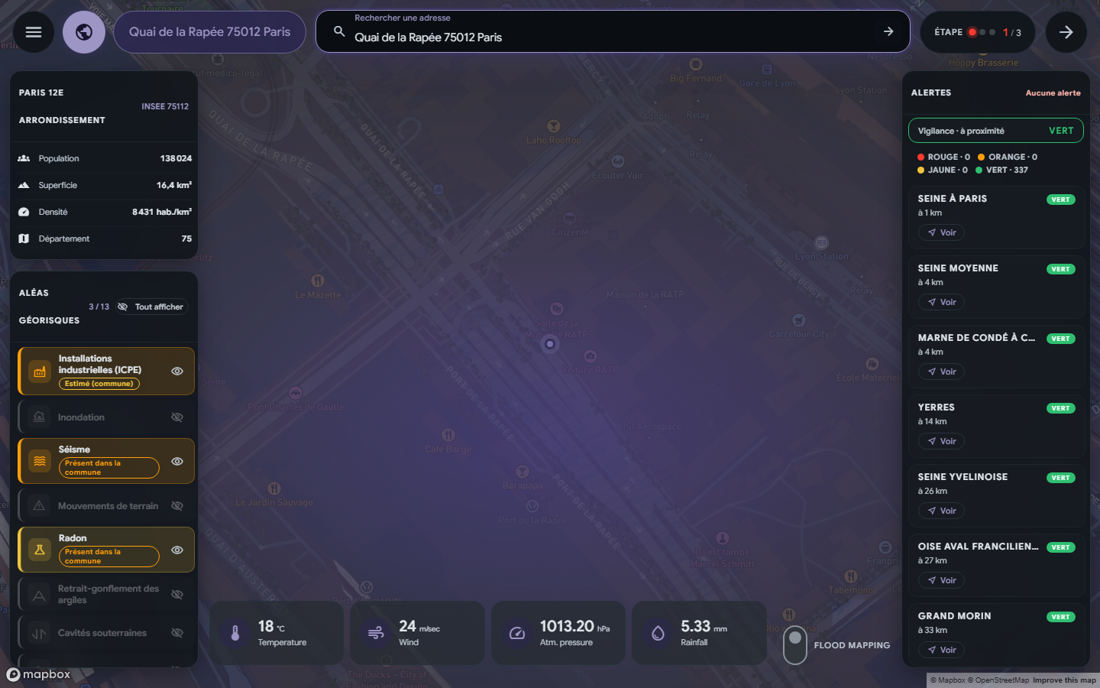
\includegraphics[width=0.95\textwidth]{../docs/screenshots/step1-diagnostic.png}
\caption{Étape 1 — diagnostic. Les 13 aléas Géorisques avec leur badge de
résolution, la fiche BDNB du bâtiment, et une photographie terrain Panoramax
orientée sur le point, sur une carte 3D.}
\label{fig:step1}
\end{figure}

\section{Le contrat en pratique}

Le contrat produit pour l'adresse de démonstration principale illustre la
jointure. On y lit, pour chaque aléa, trois informations indissociables : le
fait, sa source, et sa résolution.

\begin{table}[H]
\centering
\small
\caption{Lecture du contrat pour l'adresse de démonstration principale.}
\label{tab:lecture-contrat}
\begin{tabularx}{\textwidth}{@{}l l l X@{}}
\toprule
\textbf{Aléa} & \textbf{\code{present}} & \textbf{Résolution} & \textbf{Origine du fait} \\
\midrule
Inondation & \code{true} & \code{per-building} &
  Test point-in-polygon réussi contre le périmètre PPR inondation \\
\addlinespace
Sismicité & selon zone & \code{commune-level} &
  Zonage sismique décrétal — résolution maximale existante \\
\addlinespace
Radon & selon commune & \code{commune-level} &
  Classement de potentiel communal \\
\addlinespace
RGA & selon commune & \code{commune-level-estimate} &
  Estimation communale assumée, source vectorielle non câblée \\
\addlinespace
Feu de forêt & \code{true}/\code{false} & \code{per-building} &
  Test géométrique contre le périmètre \\
\bottomrule
\end{tabularx}
\end{table}

Le point important n'est pas la valeur de chaque ligne, mais le fait que la
troisième colonne existe. Un lecteur du contrat sait \emph{toujours} à quel
niveau l'information a été établie, et peut donc décider du crédit à lui
accorder.

\section{Ce que le produit démontre}

\subsection{La jointure existe et elle est vérifiée}

Le résultat central est que la jointure entre exposition et vulnérabilité, à
l'échelle du bâtiment, est établie par un test géométrique réel et non par une
approximation communale. Pour les aléas couverts par un périmètre vectoriel, le
fait porte effectivement sur le bâtiment.

\subsection{Le refus du score est tenable}

La suppression du score composite a été testée jusqu'au bout : le schéma refuse
la sérialisation de champs de score, une porte de recherche échoue si un tel
champ apparaît, et la valeur produit se reconstruit sur d'autres fondations —
la provenance et la résolution. Le produit est démontrable sans son chiffre.

\subsection{Les modes de défaillance sont explicites}

La trichotomie \code{true}/\code{false}/\code{null} et la matrice d'erreurs
font que le produit ne confond jamais \og pas de risque \fg{} et \og je ne sais
pas \fg. C'est peut-être la propriété la plus difficile à démontrer sur un
produit de données, et elle est ici vérifiée par une suite de tests de
dégradation.

\subsection{Le moteur de scénarios relie la donnée au jugement}

La carte ne montre pas une donnée : elle montre la jointure. Et le moteur de
scénarios transforme une classe de retour abstraite (\og 100 ans \fg) en une
montée des eaux lisible, sans jamais inventer un niveau.

\section{Chiffres clés}

\begin{table}[H]
\centering
\small
\caption{Synthèse quantitative du projet.}
\label{tab:chiffres}
\begin{tabularx}{\textwidth}{@{}l l X@{}}
\toprule
\textbf{Indicateur} & \textbf{Valeur} & \textbf{Commentaire} \\
\midrule
Commits & 76 & du 14 août au 15 septembre 2026 \\
\addlinespace
Fichiers Python (backend) & 70 & dont 10 connecteurs, 8 routes, 7 services \\
\addlinespace
Modules TypeScript (frontend) & 68 & dont 20 dans le moteur de scénarios \\
\addlinespace
Modules de test & 45 & 24 backend, 21 frontend \\
\addlinespace
Tests automatisés & 357 & 214 backend, 143 frontend, hors-ligne \\
\addlinespace
Exigences fonctionnelles & 28 & \frref{01} à \frref{28}, chacune avec
  critères d'acceptation \\
\addlinespace
Tâches planifiées & 18 + 10 & plan principal + plan de scénarios \\
\addlinespace
Aléas normalisés & 13 & référentiel Géorisques complet \\
\addlinespace
Aléas certifiés & 4 & inondation, mouvement de terrain, feu, avalanche \\
\addlinespace
Sources externes intégrées & 9 & dont 7 publiques \\
\addlinespace
Sections constitutionnelles & 8 & dont un amendement (§2.1, mode VFX) \\
\addlinespace
Décisions documentées & 13 + 5 & cadrage + moteur de scénarios \\
\bottomrule
\end{tabularx}
\end{table}

\section{Validation}

La validation du travail repose sur quatre niveaux complémentaires.

\begin{description}[leftmargin=0em,style=nextline]
  \item[Tests automatisés.] 357 tests hors-ligne, exécutés en moins d'une
  minute pour le backend. Ils couvrent le chemin nominal, la dégradation, les
  invariants de schéma et l'équivalence unitaire/lot.
  \item[Vérification en ligne.] Une instance déployée, contrôlée endpoint par
  endpoint le 15 septembre 2026 (tableau~\ref{tab:verif}).
  \item[Confrontation au métier.] Les décisions structurantes — refus du score,
  variables brutes plutôt qu'un indice, livraison à la fois interactive et en
  lot — proviennent d'échanges réels avec un actuaire et un professionnel du
  secteur, pas d'une hypothèse de conception.
  \item[Reproductibilité de la démonstration.] Trois adresses de référence
  documentées, avec le résultat attendu pour chacune, permettent de rejouer la
  démonstration à l'identique.
\end{description}

\section{Apports personnels}

Au-delà du livrable, ce stage a produit plusieurs apprentissages que je
considère transférables.

\begin{enumerate}[leftmargin=1.6em]
  \item \textbf{La valeur d'un produit de données tient à sa traçabilité, pas à
        son volume.} Une jointure modeste mais vérifiable vaut mieux qu'une
        agrégation large et approximative.
  \item \textbf{Le refus est une décision d'ingénierie.} Supprimer le score,
        supprimer quatre connecteurs, supprimer des milliers de lignes a
        \emph{augmenté} la valeur du livrable.
  \item \textbf{Une panne silencieuse est plus dangereuse qu'une erreur
        visible.} Le bug de la boîte englobante répondait correctement avec une
        information fausse. C'est ce qui m'a conduit à traiter la trichotomie
        \code{true}/\code{false}/\code{null} comme une exigence de premier rang.
  \item \textbf{Un correctif non documenté sera défait.} Travailler avec des
        agents de programmation rend cette règle vitale : l'invariant doit
        exister dans un document lu avant le code.
  \item \textbf{Les sources publiques ont des pièges non documentés.} Le client
        HTTP partagé, la boîte englobante, l'ordre des axes GML : rien de tout
        cela n'est dans la documentation officielle. Le savoir s'accumule par
        la mesure et doit être écrit.
\end{enumerate}

\section{Impact potentiel}

Il serait malhonnête de présenter \typhoon{} comme un produit prêt à être
vendu. C'est un prototype fonctionnel qui démontre une thèse : la jointure
aléa $\times$ vulnérabilité par bâtiment est réalisable à partir de sources
publiques, avec une traçabilité compatible avec les exigences d'un audit.

Le chemin vers un usage réel passe par des étapes identifiées : qualification
humaine de la certification, calibration de latence, authentification réelle,
persistance du store de lot, et surtout validation de l'intérêt par un pilote
chez un assureur. La valeur du prototype est d'avoir rendu cette discussion
concrète — on ne débat plus de l'idée, on débat d'une URL qu'on peut ouvrir.
